\documentclass[b5paper,twoside]{book}
\usepackage[lmargin=25mm,rmargin=25mm,tmargin=27mm,bmargin=30mm]{geometry}
\usepackage{lmodern}
\usepackage{amssymb,amsmath}
\usepackage{fixltx2e} % provides \textsubscript
\usepackage[T1]{fontenc}
\usepackage[utf8]{inputenc}

\usepackage{natbib}
\bibliographystyle{plain}

\usepackage{graphicx}
\usepackage{color}
\usepackage{xcolor}
\usepackage{listings}
\usepackage{chngcntr}
\usepackage[chapter]{minted}
\usepackage{url}
\usepackage{caption}
\usepackage{subcaption}

\DeclareCaptionFont{white}{\color{white}}
\DeclareCaptionFormat{listing}{\colorbox[rgb]{0.18, 0.25, 0.11}{\parbox{0.965\textwidth}{\hspace{10pt}#1#2#3}}}
\captionsetup[lstlisting]{format=listing,labelfont=white,textfont=white, singlelinecheck=false, margin=0pt, font={bf,footnotesize}}

\definecolor{lgray}{gray}{0.95}
\definecolor{dgray}{gray}{0.2}
\definecolor{keywd}{rgb}{.28,.35,.51}
\definecolor{operator}{rgb}{.28,.35,.51}

\setcounter{secnumdepth}{3}

% Style Minted
\usemintedstyle{tango}
\definecolor{codebg}{rgb}{0.98,0.97,0.97}
\newminted{sql}{bgcolor=codebg,
                    linenos=true,
                    numbersep=10pt}

\newminted{javascript}{bgcolor=codebg,
                    linenos=true,
                    numbersep=10pt}


\lstset{
    backgroundcolor=\color{white},
    basicstyle=\ttfamily\color{dgray}\footnotesize,
    linewidth=0.965\textwidth,
    belowcaptionskip=2pt,
    frame=none,
    aboveskip=20pt,
    belowskip=20pt,
    language=Java
    % language=c,
    % commentstyle={\color{gray}},
}


% use upquote if available, for straight quotes in verbatim environments
\IfFileExists{upquote.sty}{\usepackage{upquote}}{}

% use microtype if available
\IfFileExists{microtype.sty}{%
\usepackage{microtype}
\UseMicrotypeSet[protrusion]{basicmath} % disable protrusion for tt fonts
}{}

\usepackage{eso-pic,graphicx}
 \definecolor{LtGrey}{rgb}{0.575,0.575,0.575}

%  \AddToShipoutPicture*{%
%  \AtTextCenter{%
%  \makebox(0,0)[c]{\resizebox{\textwidth}{!}{%
%   \rotatebox{45}{\textsf{\textbf{\color{LtGrey}DRAFT}}}}}
% }
% }

%\usepackage[toc,page]{appendix}

\usepackage[linktocpage=true,colorlinks]{hyperref}
\hypersetup{
            pdftitle={A Very Long Title Yeah},
            pdfauthor={John Doe},
            colorlinks=true,
            linkcolor=black,
            citecolor=black,
            urlcolor=blue,
            linktoc=all,
            pdfborder={0 0 0},
            breaklinks=true
}




\usepackage{rotating,multirow,longtable,booktabs}
% % Fix footnotes in tables (requires footnote package)
\IfFileExists{footnote.sty}{\usepackage{footnote}\makesavenoteenv{long table}}{}
\usepackage{graphicx,grffile}
\makeatletter
\def\maxwidth{\ifdim\Gin@nat@width>\linewidth\linewidth\else\Gin@nat@width\fi}
\def\maxheight{\ifdim\Gin@nat@height>\textheight\textheight\else\Gin@nat@height\fi}
\makeatother
% Scale images if necessary, so that they will not overflow the page
% margins by default, and it is still possible to overwrite the defaults
% using explicit options in \includegraphics[width, height, ...]{}
\setkeys{Gin}{width=\maxwidth,height=\maxheight,keepaspectratio}

\setlength{\emergencystretch}{3em}  % prevent overfull lines
\providecommand{\tightlist}{%
  \setlength{\itemsep}{0pt}\setlength{\parskip}{0pt}}

\setlength{\parindent}{0em}
\setlength{\parskip}{1em}

%
% % \setcounter{secnumdepth}{0}
% 

\usepackage[acronym]{glossaries}
\makeglossaries

\newglossaryentry{latex}
{
    name=latex,
    description={Is a mark up language specially suited
    for scientific documents}
}

\newglossaryentry{maths}
{
    name=mathematics,
    description={Mathematics is what mathematicians do}
}

\newacronym{lvm}{LVM}{Logical Volume Manager}
\newacronym{IDI}{IDI}{Department of Computer and Information Science}
\newacronym{NTNU}{NTNU}{Norwegian University of Science and Technology}


% set default figure placement to htbp
\makeatletter
\def\fps@figure{htbp}
\makeatother


\begin{document}
\pagenumbering{roman}
\begin{titlepage}

\begin{center}
    
\includegraphics[height=1.5cm]{images/ntnu-logo.pdf}\\[1cm] %or company logo etc.
\end{center}
\begin{center}

% Upper part of the page
~\\[1.5cm]

\textsc{\Large Master Thesis }\\[0.5cm]

% Set the title of the Document between two horizontal lines
\hrule ~\\[0.4cm]
{\huge \bfseries A Very Long
Title Yeah}\\[0.5cm]		% print the title of the document
\hrule ~\\[1.5cm]

% Additional Information about the document
\begin{minipage}{0.4\textwidth}
  \centering
	  \large
		  John Doe\\
		  \vspace{2.5cm}
		  \vspace{1.5cm}
		  \textbf{Supervisor:}  \\ David Webb %add other people in a similar way
\end{minipage}

\vfill

% Bottom of the page
{\large Fall 2016}

\thispagestyle{empty}

\end{center}
\end{titlepage}

\setcounter{page}{0}
\chapter*{Abstract}
\addcontentsline{toc}{chapter}{Abstract}
Abstract in english


\chapter*{Sammendrag}
\addcontentsline{toc}{chapter}{Sammendrag}
Sammendrag på norsk


\chapter*{Preface}
\addcontentsline{toc}{chapter}{Preface}
This is cool.


\tableofcontents
\addcontentsline{toc}{chapter}{Table of Contents}
\clearpage

\listoftables
\addcontentsline{toc}{chapter}{List of Tables}
\clearpage

\listoffigures
\addcontentsline{toc}{chapter}{List of Figures}
\clearpage

\addcontentsline{toc}{chapter}{Abbreviations}
\printglossaries
\clearpage

\pagenumbering{arabic}

\chapter{Introduction}\label{introduction}

It is very easy
to write stuff
in Markdown.
Writing reports
is something you
do a lot a
places like
\gls{NTNU}. You
won't believe it
\citep{vg}.

\section{I'll
Make a
List}\label{ill-make-a-list}

\begin{itemize}
\tightlist
\item
  This
\item
  Is
\item
  So
\item
  Awesome\footnote{Yes,
    it is.}.
\item
  Figure
  \ref{bourne}
  shows a
  picture of
  Jason Bourne.
\end{itemize}

\begin{figure}
\centering
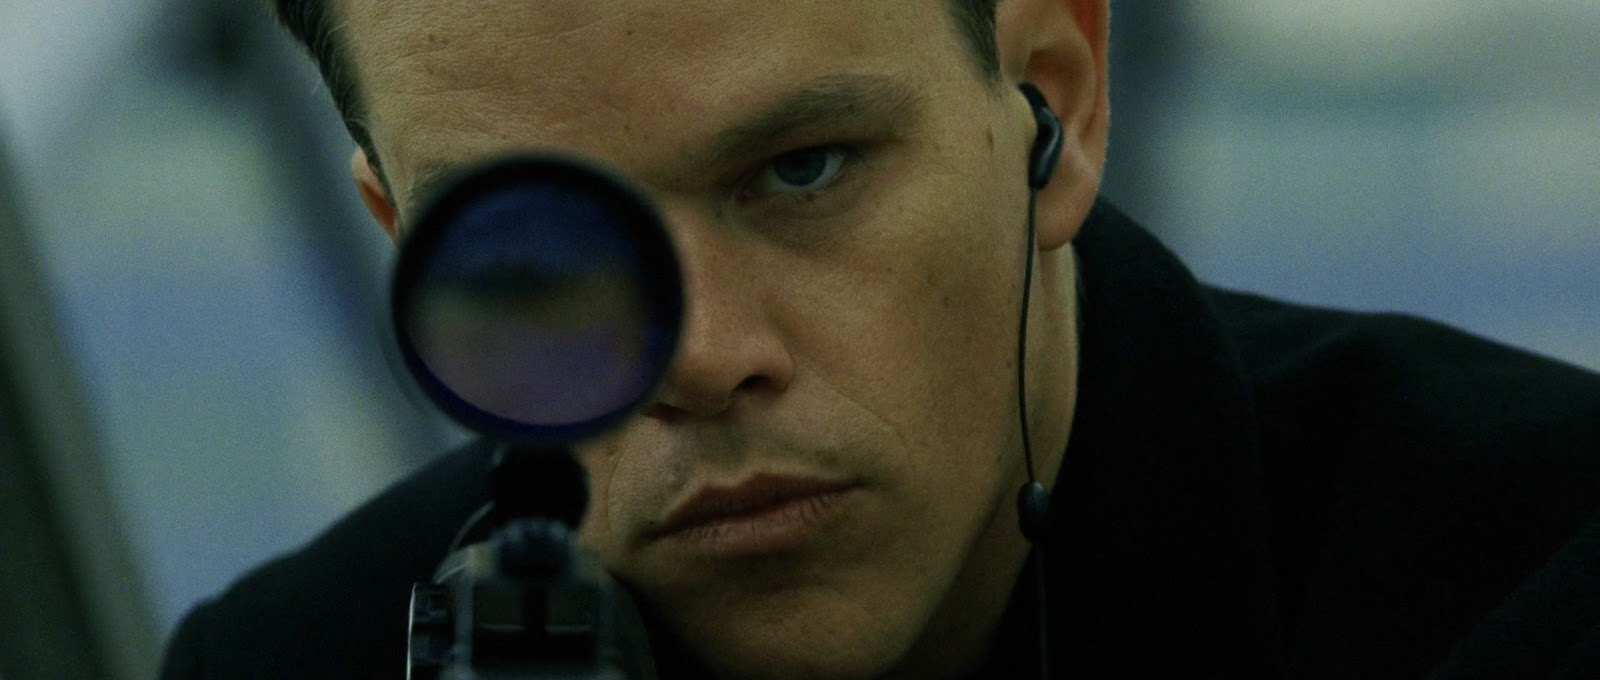
\includegraphics{images/jason-bourne.jpg}
\caption{Jason
Bourne\label{bourne}}
\end{figure}

\chapter{Background}\label{background}

\chapter{Research
Methodology}\label{research-methodology}

He-he-he

\renewcommand\bibname{Bibliography}

\bibliography{references}


\end{document}
